\subsection{RGB Konvertierung}

Für die Analyse des CMBs werden die sphärischen harmonische Koeffizienten 
$c_l^m$ benötigt. Dafür müssen aber erst die Bilddaten, welche im Rot-Grün-Blau 
(RGB) Format vorliegen, in Kelvin Werte umgewandelt werden. Da nicht klar ist, 
wie genau die ursprüngliche Transformation aussah, wird die Analyse mittels 
einer Annäherung an die wirkliche Transformationsfunktion durchgeführt.

Den dafür benötigten Referenzfarbverlauf finden wir in den Resultaten der 
Planck Mission \cite{cmb:planck_overview}, zu sehen in 
Abbildung~\ref{fig:rgb-profiles}~(a). Ein Blick auf die einzelnen RGB 
Kanäle in Abbildung~\ref{fig:rgb-profiles}~(c) zeigt, wie eine mögliche 
Funktion aussehen könnte. Da es dabei aber um einen Screenshot 
der im PDF Dokument enthaltenen Grafik handelt, ist die Farbtreue nicht gegeben 
und somit ist auch dies nicht die echte Transformationsfunktion. Als mögliche 
Annäherung wird daher der Farbverlauf in Abbildung~\ref{fig:rgb-profiles}~(b) 
verwendet. Betrachtet man dessen RGB-Profil in 
Abbildung~\ref{fig:rgb-profiles}~(d), so hat dies den Vorteil, dass man die 
einzelnen Kanäle aufsummieren kann und zwei einfache lineare Funktionen
\begin{equation*}
	y =
	\begin{dcases}
		\frac{765}{500}x + 765 & \text{für} \quad x \leq 0,\\
		-\frac{765}{500}x + 765 & \text{für} \quad x \geq 0,\\
	\end{dcases}
\end{equation*}
erhält. Da wir ja die $y$-Werte kennen, müssen wir die Funktion umkehren, 
was uns
\begin{align*}
	x_1 &= 500\frac{y - 765}{765}\\
	x_2 &= -500\frac{y - 765}{765}
\end{align*}
liefert. Um die beiden Fälle zu unterscheiden, genügt es, lediglich den Anteil 
des blauen und roten Kanals miteinander zu vergleichen. Enthält ein Pixel mehr 
Rot als Blau gilt die Formel für $x_2$ andernfalls diejenige für $x_1$.

\begin{figure}
	\centering
	\subfigure[Farbverlauf der ESA Planck Missions CMB Bilder.]{
		
\includegraphics[width=0.48\textwidth]{cmb/images/color-strip-full.png}
	}
	\subfigure[Der für die Analyse verwendete Farbverlauf.]{
		
\includegraphics[width=0.48\textwidth]{cmb/converter/converter-function-strip.png}
	}
	\subfigure[RGB Profil des Farbverlaufs in (a)]{
		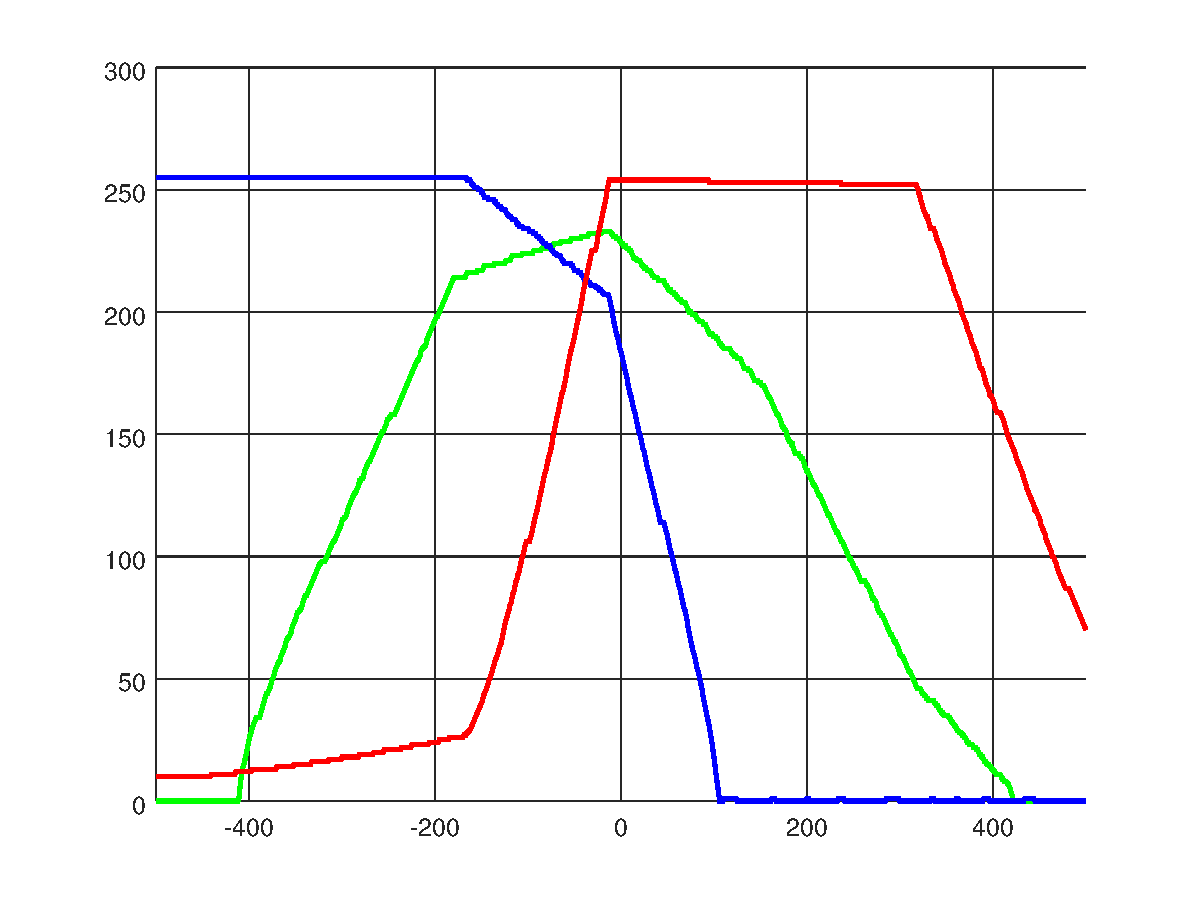
\includegraphics[width=0.48\linewidth]{cmb/converter/rgb-graph.pdf}
	}
	\subfigure[RGB Profil des Farbverlaufs in (b)]{
		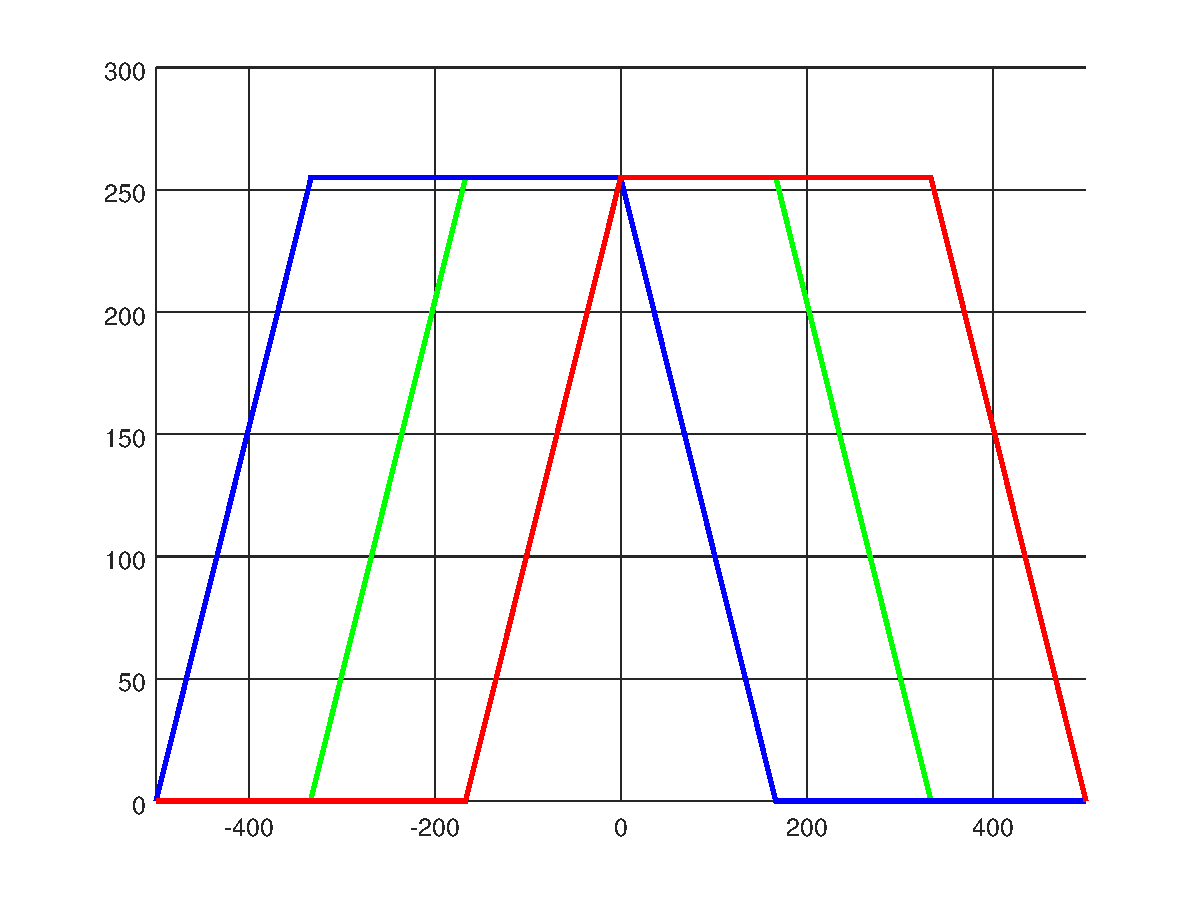
\includegraphics[width=0.48\linewidth]{cmb/converter/converter-function.pdf}
	}
	\caption{Farbverlauf der für die Codierung der CMB Bilder verwendet wird 
	zusammen mit den entsprechenden RGB Profilen. Die Farbverläufe stehen dabei 
	für eine Temperaturabweichung von $-500\mu\text{K}$ bis $500\mu\text{K}$. 
	Verlauf (a) wurde im originalen Bild verwendet. Für die Rücktransformation 
	der Verlauf (b) genutzt.}
	\label{fig:rgb-profiles}
\end{figure}
